%---------change this every homework
\def\yourid{mst3k}  % substitute your userid
\def\collabs{collaborators} % substitute your collaborators
\def\sources{sources} % substitute your sources
% -----------------------------------------------------
\def\duedate{September 10, 2025 at 11:59 pm}
\def\pnumber{1}
%-------------------------------------

\documentclass[10pt]{article}
\usepackage{dsa2}

\begin{document}
\thispagestyle{empty}
\handout



%----Begin your modifications here

%%%%%%%%%%%%%%%%%%%%%%%%%%%%%%%%%%%%%%%%%%%%%%%%%%%%%%%%
\begin{problem} Proving Complexity \end{problem}

Given the following functions, $f(n)=5n^3 + 8n^2 - 3n + 14$ and $g(n)=n^3$.

\begin{enumerate}
    \item Show that $f(n) = \Theta(g(n))$ using a direct proof, as shown in lecture. Choose integer values for $n_0$ and $c$ that are low, or about as low, as possible.

    \solution{
        % Your solution here
    }

    \item Using the limit definitions, show which of the complexity classes $f(n)$ is in relative to $g(n)$.  In other words, show whether $f(n)=\Omega(g(n))$, and similarly for the other complexity classes ($O$, $\Theta$, $o$, $\omega$).

    \solution{
        $\lim_{n\rightarrow\infty} \frac{f(n)}{g(n)} = ...$
        % Start with the line above and continue here
    }

\end{enumerate}

%%%%%%%%%%%%%%%%%%%%%%%%%%%%%%%%%%%%%%%%%%%%%%%%%%%%%%%%
\begin{problem} Graph Representations \end{problem}

Consider the following weighted digraph:

    %%%%%%%%%%% START GRAPH
    \vskip 2em
    \begin{center}
    \resizebox{.45\textwidth}{!}{\begin{tikzpicture}[->,>=stealth',shorten >=1pt,auto,node distance=3cm,thick,main node/.style={circle,fill=gray!10,draw,
      font=\sffamily\Large\bfseries,minimum size=10mm}]

      \node[main node] (a) {a};
      \node[main node] (g) [left of=a] {g};
      \node[main node] (b) [right of=a] {b};
      \node[main node] (e) [above of=b] {e};
      \node[main node] (d) [right of=b] {d};
      \node[main node] (c) [above of=a] {c};
      \node[main node] (f) [left of=c] {f};

      \path[every node/.style={
            fill=white,inner sep=2pt}]
        (a) edge [] node[] {7} (b)
            edge [] node[] {6} (c)
        (b) edge [] node[] {1} (d)
            edge [] node[] {9} (e)
        (c) edge [] node[] {3} (f)
            edge [] node[] {6} (e)
        (d) edge [bend right] node[] {2} (e)
            edge [bend left] node[] {2} (g)
        (e) edge [bend right] node[] {6} (f)
            edge [] node[] {4} (a)
        (f) edge [] node[] {8} (g)
        (g) edge [] node[] {9} (a)
        ;
    \end{tikzpicture}}\hfill

    \end{center}
    \hspace{2.2 in} Graph $G$
    %%%%%%%%%%% END GRAPH


    \begin{enumerate}
    \item Show a representation of this graph using an adjacency matrix. Your representation should look similar in format to the adjacency matrix shown in lecture. The format of a graph is given to you as a starting point. If no edge exists, leave the cell blank. The number "2025" has been placed in the first cell just to show you where to modify cell values. Remove it and either leave it blank or replace it with a value if appropriate.

    \solution{

    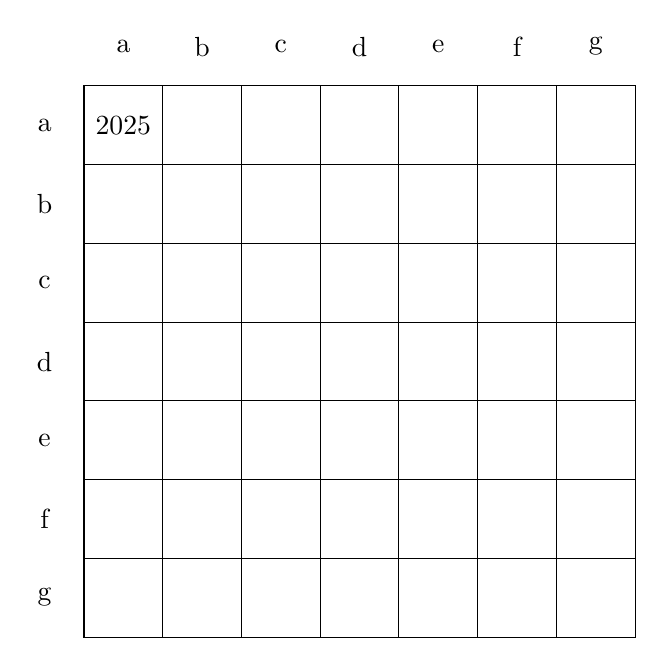
\begin{tikzpicture}

    % Label rows and columns
    \node at (-0.5, -0.5) {a};
    \node at (-0.5, -1.5) {b};
    \node at (-0.5, -2.5) {c};
    \node at (-0.5, -3.5) {d};
    \node at (-0.5, -4.5) {e};
    \node at (-0.5, -5.5) {f};
    \node at (-0.5, -6.5) {g};

    \node at (0.5, 0.5) {a};
    \node at (1.5, 0.5) {b};
    \node at (2.5, 0.5) {c};
    \node at (3.5, 0.5) {d};
    \node at (4.5, 0.5) {e};
    \node at (5.5, 0.5) {f};
    \node at (6.5, 0.5) {g};

    % Draw the grid and fill with question marks.
    % Enter a value at the end of each row in the curly braces as appropriate. 
    % bRecompile after modifying to make sure you did what you expected.

    % row a
    \draw (0, 0) rectangle (1, -1); \node at (0.5, -0.5) {2025};
    \draw (1, 0) rectangle (2, -1); \node at (1.5, -0.5) {};
    \draw (2, 0) rectangle (3, -1); \node at (2.5, -0.5) {};
    \draw (3, 0) rectangle (4, -1); \node at (3.5, -0.5) {};
    \draw (4, 0) rectangle (5, -1); \node at (4.5, -0.5) {};
    \draw (5, 0) rectangle (6, -1); \node at (5.5, -0.5) {};
    \draw (6, 0) rectangle (7, -1); \node at (6.5, -0.5) {};

    % row b
    \draw (0, -1) rectangle (1, -2); \node at (0.5, -1.5) {};
    \draw (1, -1) rectangle (2, -2); \node at (1.5, -1.5) {};
    \draw (2, -1) rectangle (3, -2); \node at (2.5, -1.5) {};
    \draw (3, -1) rectangle (4, -2); \node at (3.5, -1.5) {};
    \draw (4, -1) rectangle (5, -2); \node at (4.5, -1.5) {};
    \draw (5, -1) rectangle (6, -2); \node at (5.5, -1.5) {};
    \draw (6, -1) rectangle (7, -2); \node at (6.5, -1.5) {};

    % row c
    \draw (0, -2) rectangle (1, -3); \node at (0.5, -2.5) {};
    \draw (1, -2) rectangle (2, -3); \node at (1.5, -2.5) {};
    \draw (2, -2) rectangle (3, -3); \node at (2.5, -2.5) {};
    \draw (3, -2) rectangle (4, -3); \node at (3.5, -2.5) {};
    \draw (4, -2) rectangle (5, -3); \node at (4.5, -2.5) {};
    \draw (5, -2) rectangle (6, -3); \node at (5.5, -2.5) {};
    \draw (6, -2) rectangle (7, -3); \node at (6.5, -2.5) {};

    % row d
    \draw (0, -3) rectangle (1, -4); \node at (0.5, -3.5) {};
    \draw (1, -3) rectangle (2, -4); \node at (1.5, -3.5) {};
    \draw (2, -3) rectangle (3, -4); \node at (2.5, -3.5) {};
    \draw (3, -3) rectangle (4, -4); \node at (3.5, -3.5) {};
    \draw (4, -3) rectangle (5, -4); \node at (4.5, -3.5) {};
    \draw (5, -3) rectangle (6, -4); \node at (5.5, -3.5) {};
    \draw (6, -3) rectangle (7, -4); \node at (6.5, -3.5) {};

    % row e
    \draw (0, -4) rectangle (1, -5); \node at (0.5, -4.5) {};
    \draw (1, -4) rectangle (2, -5); \node at (1.5, -4.5) {};
    \draw (2, -4) rectangle (3, -5); \node at (2.5, -4.5) {};
    \draw (3, -4) rectangle (4, -5); \node at (3.5, -4.5) {};
    \draw (4, -4) rectangle (5, -5); \node at (4.5, -4.5) {};
    \draw (5, -4) rectangle (6, -5); \node at (5.5, -4.5) {};
    \draw (6, -4) rectangle (7, -5); \node at (6.5, -4.5) {};

    % row f
    \draw (0, -5) rectangle (1, -6); \node at (0.5, -5.5) {};
    \draw (1, -5) rectangle (2, -6); \node at (1.5, -5.5) {};
    \draw (2, -5) rectangle (3, -6); \node at (2.5, -5.5) {};
    \draw (3, -5) rectangle (4, -6); \node at (3.5, -5.5) {};
    \draw (4, -5) rectangle (5, -6); \node at (4.5, -5.5) {};
    \draw (5, -5) rectangle (6, -6); \node at (5.5, -5.5) {};
    \draw (6, -5) rectangle (7, -6); \node at (6.5, -5.5) {};

    % row g
    \draw (0, -6) rectangle (1, -7); \node at (0.5, -6.5) {};
    \draw (1, -6) rectangle (2, -7); \node at (1.5, -6.5) {};
    \draw (2, -6) rectangle (3, -7); \node at (2.5, -6.5) {};
    \draw (3, -6) rectangle (4, -7); \node at (3.5, -6.5) {};
    \draw (4, -6) rectangle (5, -7); \node at (4.5, -6.5) {};
    \draw (5, -6) rectangle (6, -7); \node at (5.5, -6.5) {};
    \draw (6, -6) rectangle (7, -7); \node at (6.5, -6.5) {};

    \end{tikzpicture}
    } % end solution

    \vspace{0.5 in}

    \item Show a representation of this graph using an adjacency list. Your representation should look similar in format to the adjacency list shown in lecture. Example formatting in given to you below.  Within each list node, the node letter is first, followed by the edge cost.

    \solution{

    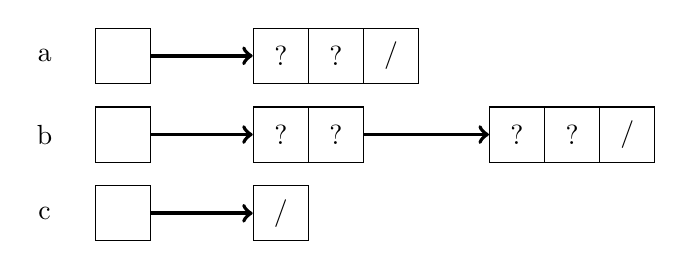
\begin{tikzpicture}

    % Below are three examples, with different number of nodes in the adjacency list 

    % Row a
    % Draw row label
    \node (label_a) at (-1,  0) {a};
    % Draw node for list index
    \node[draw, rectangle, minimum width=0.7cm, minimum height=0.7cm] (a0) at (0,  0) {};
    % Draw list nodes with three elements (the last being the null pointer)
    \node[draw, rectangle, minimum width=0.7cm, minimum height=0.7cm] (a0_1a) at (2, 0) {?};
    \node[draw, rectangle, minimum width=0.7cm, minimum height=0.7cm] (a0_1b) at (2.7, 0) {?};
    \node[draw, rectangle, minimum width=0.7cm, minimum height=0.7cm] (a0_1c) at (3.4, 0) {/};
    % Draw arrow connecting index to first nodes
    \draw[->, line width=0.5mm] (a0.east) -- (a0_1a.west);

    % Row b
    % Draw row label
    \node (label_b) at (-1, -1) {b};
    % Draw node for list index
    \node[draw, rectangle, minimum width=0.7cm, minimum height=0.7cm] (b0) at (0, -1) {};
    % Draw list node with two elements (and an outgoing pointer)
    \node[draw, rectangle, minimum width=0.7cm, minimum height=0.7cm] (b0_1a) at (2, -1) {?};
    \node[draw, rectangle, minimum width=0.7cm, minimum height=0.7cm] (b0_1b) at (2.7, -1) {?};
    % Draw arrow connecting first list node to second list node
    \draw[->, line width=0.5mm] (b0.east) -- (b0_1a.west);
    % Draw list nodes with three elements (the last being the null pointer)
    \node[draw, rectangle, minimum width=0.7cm, minimum height=0.7cm] (b0_2a) at (5, -1) {?};
    \node[draw, rectangle, minimum width=0.7cm, minimum height=0.7cm] (b0_2b) at (5.7, -1) {?};
    \node[draw, rectangle, minimum width=0.7cm, minimum height=0.7cm] (b0_2c) at (6.4, -1) {/};
    % Draw arrow connecting first list node to second list node
    \draw[->, line width=0.5mm] (b0_1b.east) -- (b0_2a.west);

    % Row c
    % Draw row label
    \node (label_c) at (-1, -2) {c};
    % Draw node for list index
    \node[draw, rectangle, minimum width=0.7cm, minimum height=0.7cm] (c0) at (0, -2) {};
    % Draw a single cell which is the null pointer
    \node[draw, rectangle, minimum width=0.7cm, minimum height=0.7cm] (c0_1a) at (2, -2) {/};
    % Draw arrow connecting index to first nodes
    \draw[->, line width=0.5mm] (c0.east) -- (c0_1a.west);

    \end{tikzpicture}

    } % end solution

\end{enumerate}


%%%%%%%%%%%%%%%%%%%%%%%%%%%%%%%%%%%%%%%%%%%%%%%%%%%%%%%%
\begin{problem} BFS vs. DFS \end{problem}

Given the following unweighted digraph:

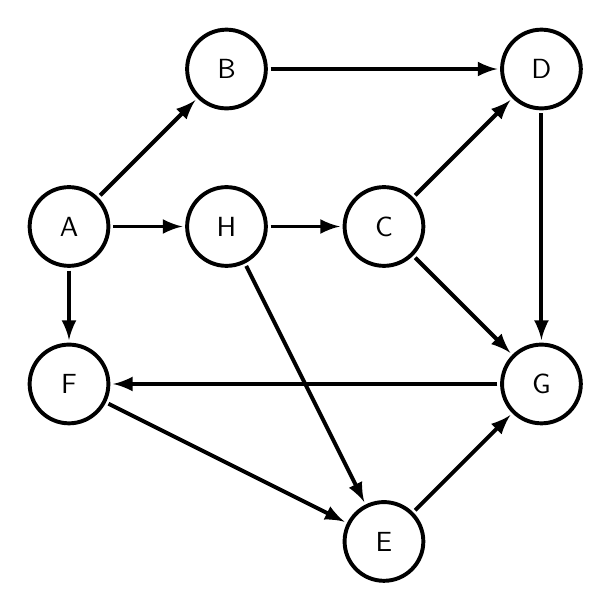
\begin{tikzpicture}[node distance=2cm,
    every node/.style={draw, circle, minimum size=1cm, font=\sffamily},
    >={latex}, line width=0.5mm, % Increase arrow line width
    shorten >=1pt, shorten <=1pt
    ]

    % Define nodes
    \node (A) at (0, 0) {A};
    \node (B) at (2, 2) {B};
    \node (C) at (4, 0) {C};
    \node (D) at (6, 2) {D};
    \node (G) at (6, -2) {G};
    \node (H) at (2, 0) {H};
    \node (E) at (4, -4) {E};
    \node (F) at (0, -2) {F};

    % Draw directed edges
    \draw[->] (A) -- (B);
    \draw[->] (A) -- (F);
    \draw[->] (B) -- (D);
    \draw[->] (C) -- (D);
    \draw[->] (C) -- (G);
    \draw[->] (D) -- (G);
    \draw[->] (F) -- (E);
    \draw[->] (H) -- (E);
    \draw[->] (H) -- (C);
    \draw[->] (E) -- (G);
    \draw[->] (G) -- (F);
    \draw[->] (A) -- (H);

\end{tikzpicture}

\begin{enumerate}
    \item Perform a breadth first search starting with node A. List the nodes visited in order of when they are first visited. Note: if multiple nodes are enqueued onto the queue in a single step, enqueue them alphabetically (i.e. If both nodes F and H follow node C, enqueue F before H).

    \solution{
        % your solution here
    }

    \item Perform a depth first search starting with node A. List the nodes visited in order of when they are first visited. Note: if multiple nodes are enqueued onto the queue in a single step, enqueue them alphabetically (i.e. If both nodes F and H follow node C, enqueue F before H).

    \solution{
        % your solution here
    }

\end{enumerate}


%%%%%%%%%%%%%%%%%%%%%%%%%%%%%%%%%%%%%%%%%%%%%%%%%%%%%%%%



\end{document}
